\documentclass[border=6pt]{standalone}
\usepackage[T1]{fontenc}
\usepackage[utf8]{inputenc}
\usepackage[scaled=0.98]{helvet}
\renewcommand{\familydefault}{\sfdefault}
\usepackage{amsmath}
\usepackage{graphicx}
\graphicspath{{../../../../../../exercises_lecturenotes/lecture_notes/kurs100_lektionsnoter/}}
\usepackage{tikz}
\usepackage{pgfplots}
\pgfplotsset{compat=1.18}
\usetikzlibrary{arrows.meta, decorations.pathreplacing, calc, positioning, fit, backgrounds, shapes.geometric}
\usepgfplotslibrary{groupplots,fillbetween}
\definecolor{scanpink}{HTML}{E5006D}
\definecolor{scanteal}{HTML}{00A6A6}
\definecolor{scannavy}{HTML}{243746}
\definecolor{scanlightgray}{HTML}{F1F2F3}
\begin{document}
    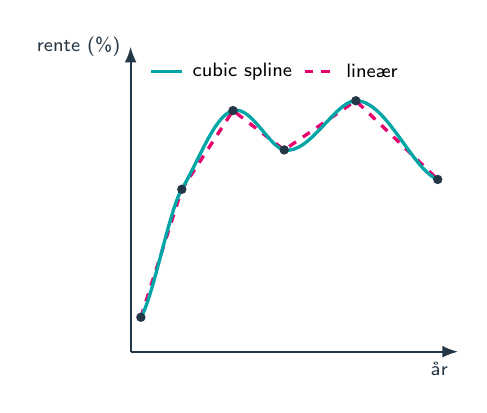
\begin{tikzpicture}[x=0.13cm,y=1.25cm,font=\scriptsize]
      \draw[-{Latex[length=2mm]},thick,scannavy] (0,0) -- (32,0) node[below left] {år};
      \draw[-{Latex[length=2mm]},thick,scannavy] (0,0) -- (0,3.1) node[left] {rente (\%)};
      \draw[very thick,scanpink,dashed]
        plot coordinates {(1,.35)(5,1.65)(10,2.45)(15,2.05)(22,2.55)(30,1.75)};
      \draw[very thick,scanteal]
        (1,.35)
        .. controls (2.2,.55) and (3.8,1.45) .. (5,1.65)
        .. controls (6.7,1.95) and (8.2,2.40) .. (10,2.45)
        .. controls (11.8,2.50) and (13.5,2.08) .. (15,2.05)
        .. controls (17.5,2.00) and (20.0,2.55) .. (22,2.55)
        .. controls (25.0,2.55) and (27.5,1.85) .. (30,1.75);
      \foreach \x/\y in {1/.35,5/1.65,10/2.45,15/2.05,22/2.55,30/1.75}
        \fill[scannavy] (\x,\y) circle (1.7pt);
      \draw[very thick,scanteal] (2,2.85)--(5,2.85) node[right,black] {cubic spline};
      \draw[very thick,scanpink,dashed] (17,2.85)--(20,2.85) node[right,black] {lineær};
    \end{tikzpicture}
\end{document}
